\documentclass{article}
\usepackage{style-notes}

\title{MATH 321: Mathematical Statistics\\Completed Notes}
\author{Colton Gearhart}
\date{\today}							

\begin{document}
\setcounter{secnumdepth}{0}		% trick to get unnumbered sections in table of contents
\maketitle
\dosecttoc
\tableofcontents
\newpage

%-------------------------------------------------------------------------
\section{Test 1}
%-------------------------------------------------------------------------

\secttoc

%%----------------------------
%\subsection{Lecture 0 -- Course Overview}
%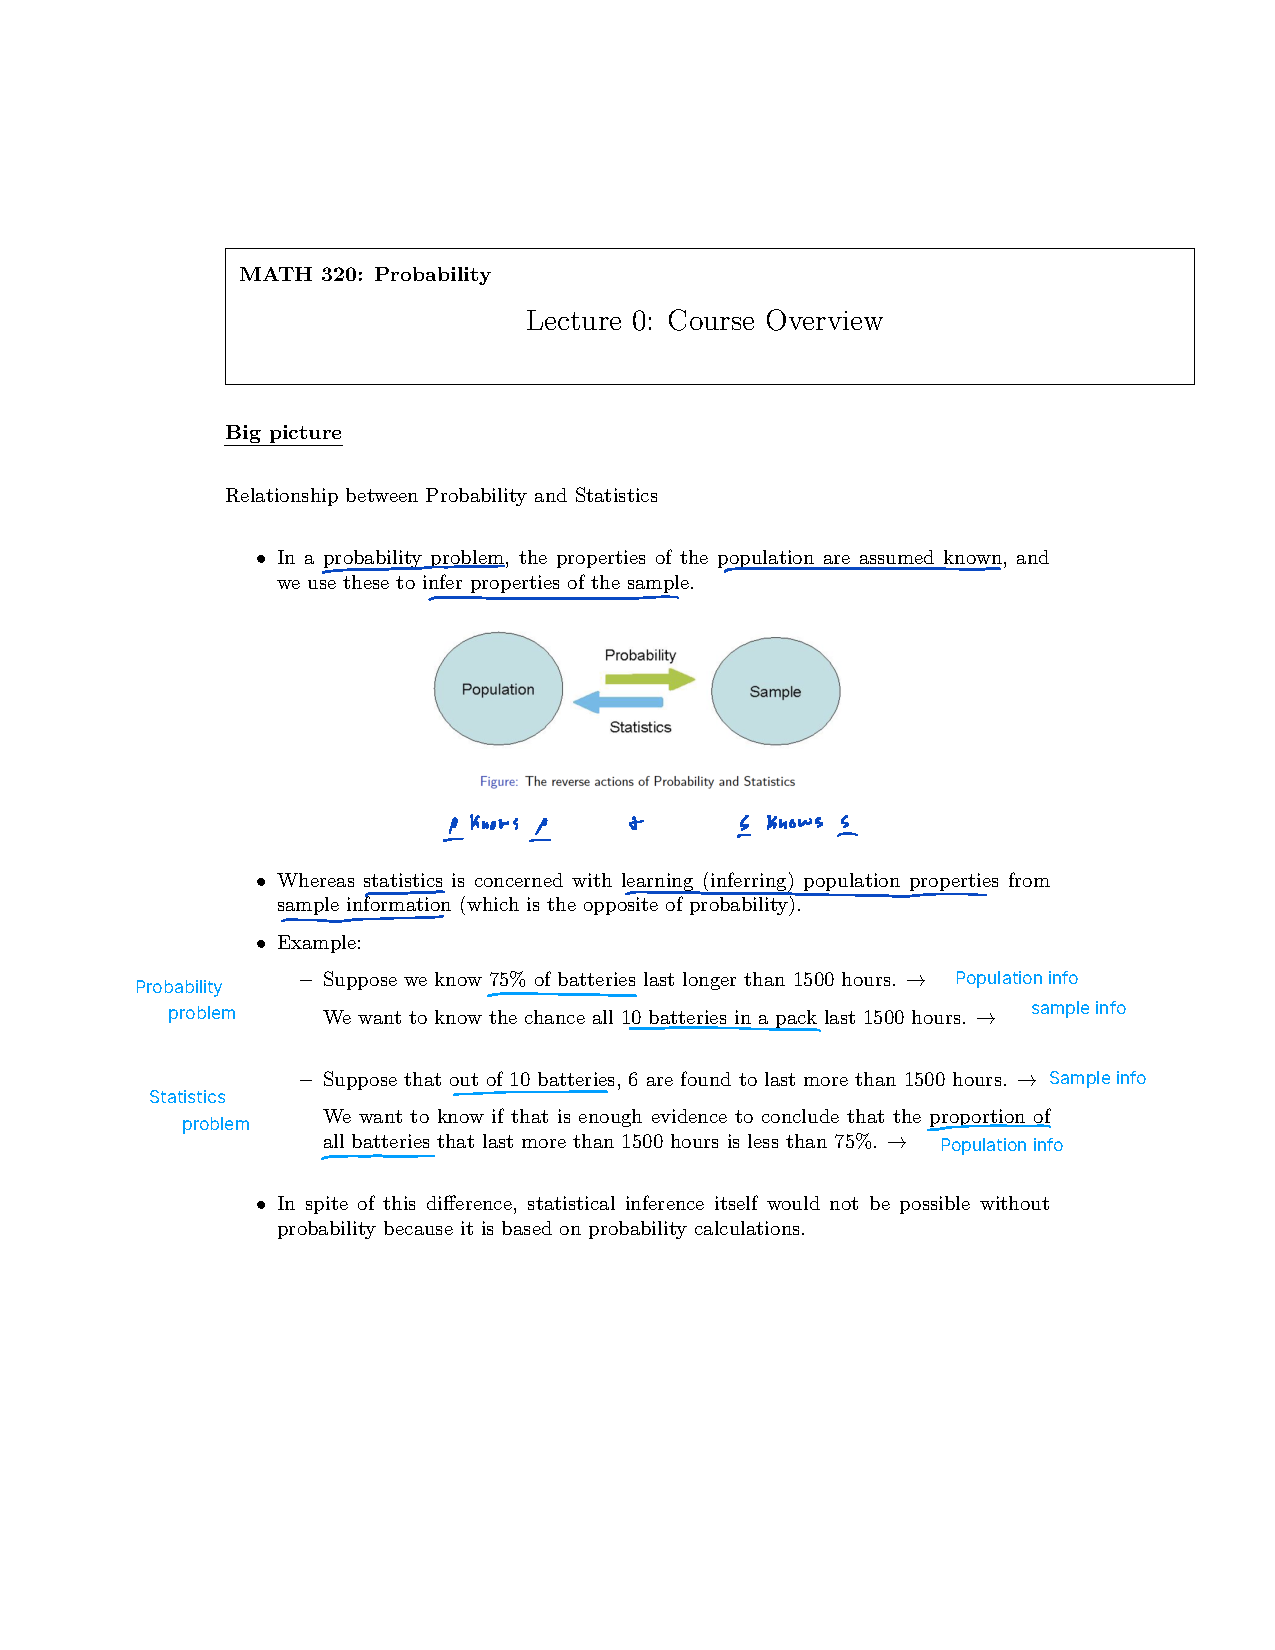
\includepdf[pages=-]{lecture-0-COMPLETED.pdf}\newpage
%%----------------------------
%
%%----------------------------
%\subsection{Lecture 1 -- XXX}
%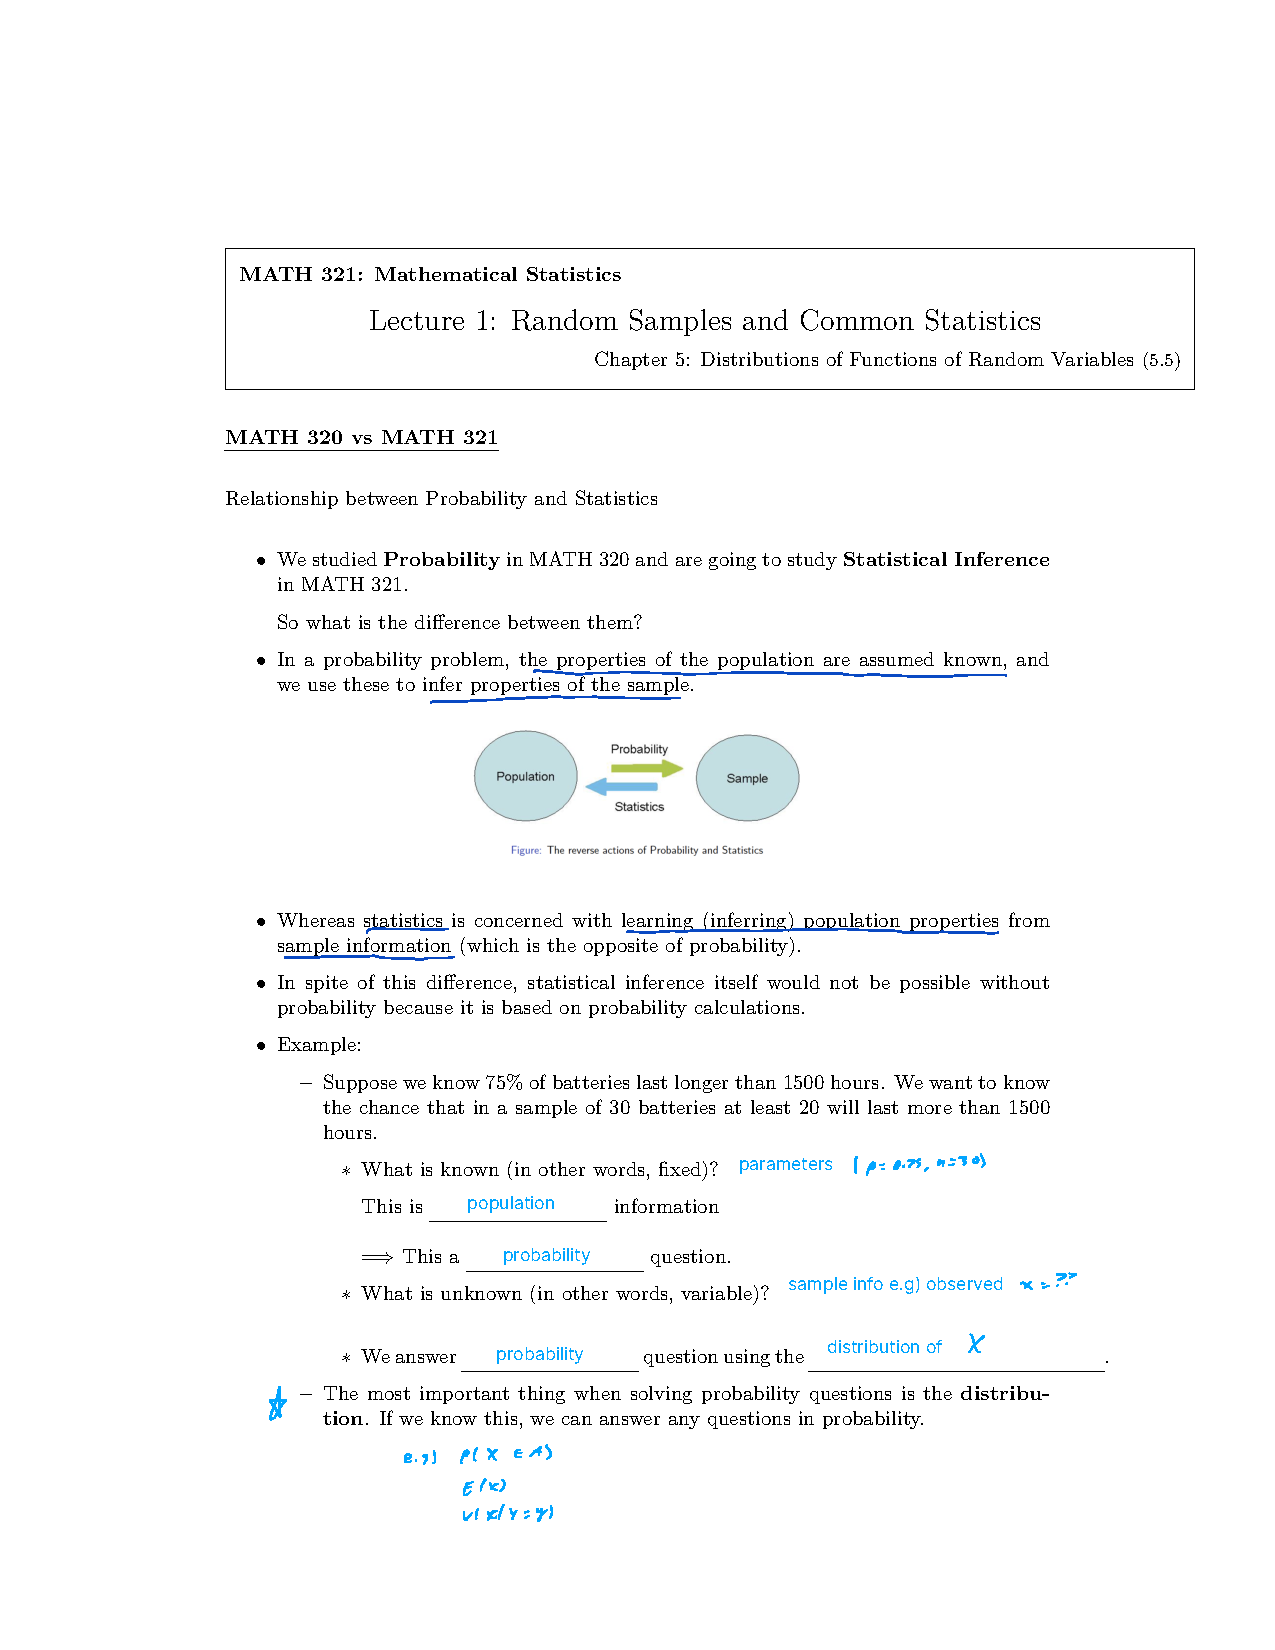
\includepdf[pages=-]{lecture-1-COMPLETED.pdf}\newpage
%%----------------------------
%
%%----------------------------
%\subsection{Lecture 2 -- XXX}
%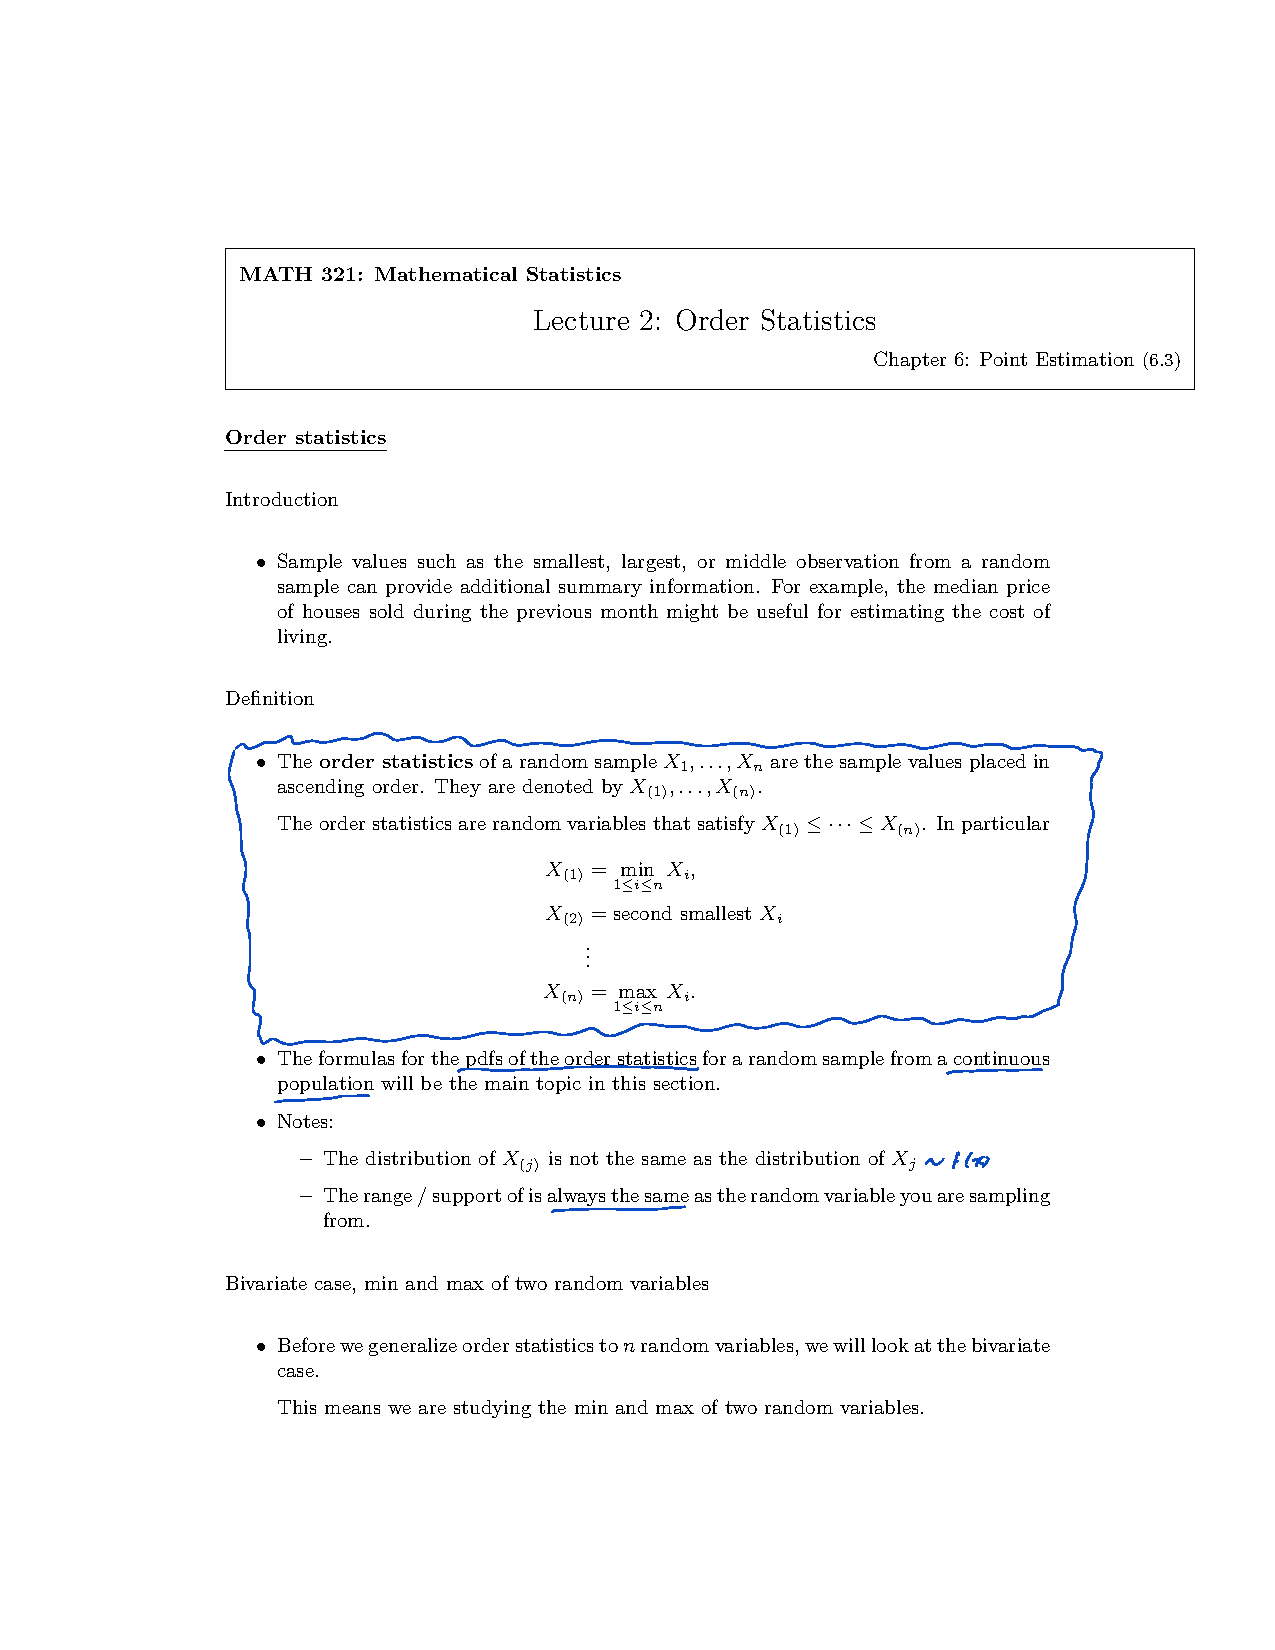
\includepdf[pages=-]{lecture-2-COMPLETED.pdf}\newpage
%%----------------------------
%
%%----------------------------
%\subsection{Lecture 3 -- XXX}
%\includepdf[pages=-]{lecture-3-COMPLETED.pdf}\newpage
%%----------------------------
%
%%----------------------------
%\subsection{Lecture 4 -- XXX}
%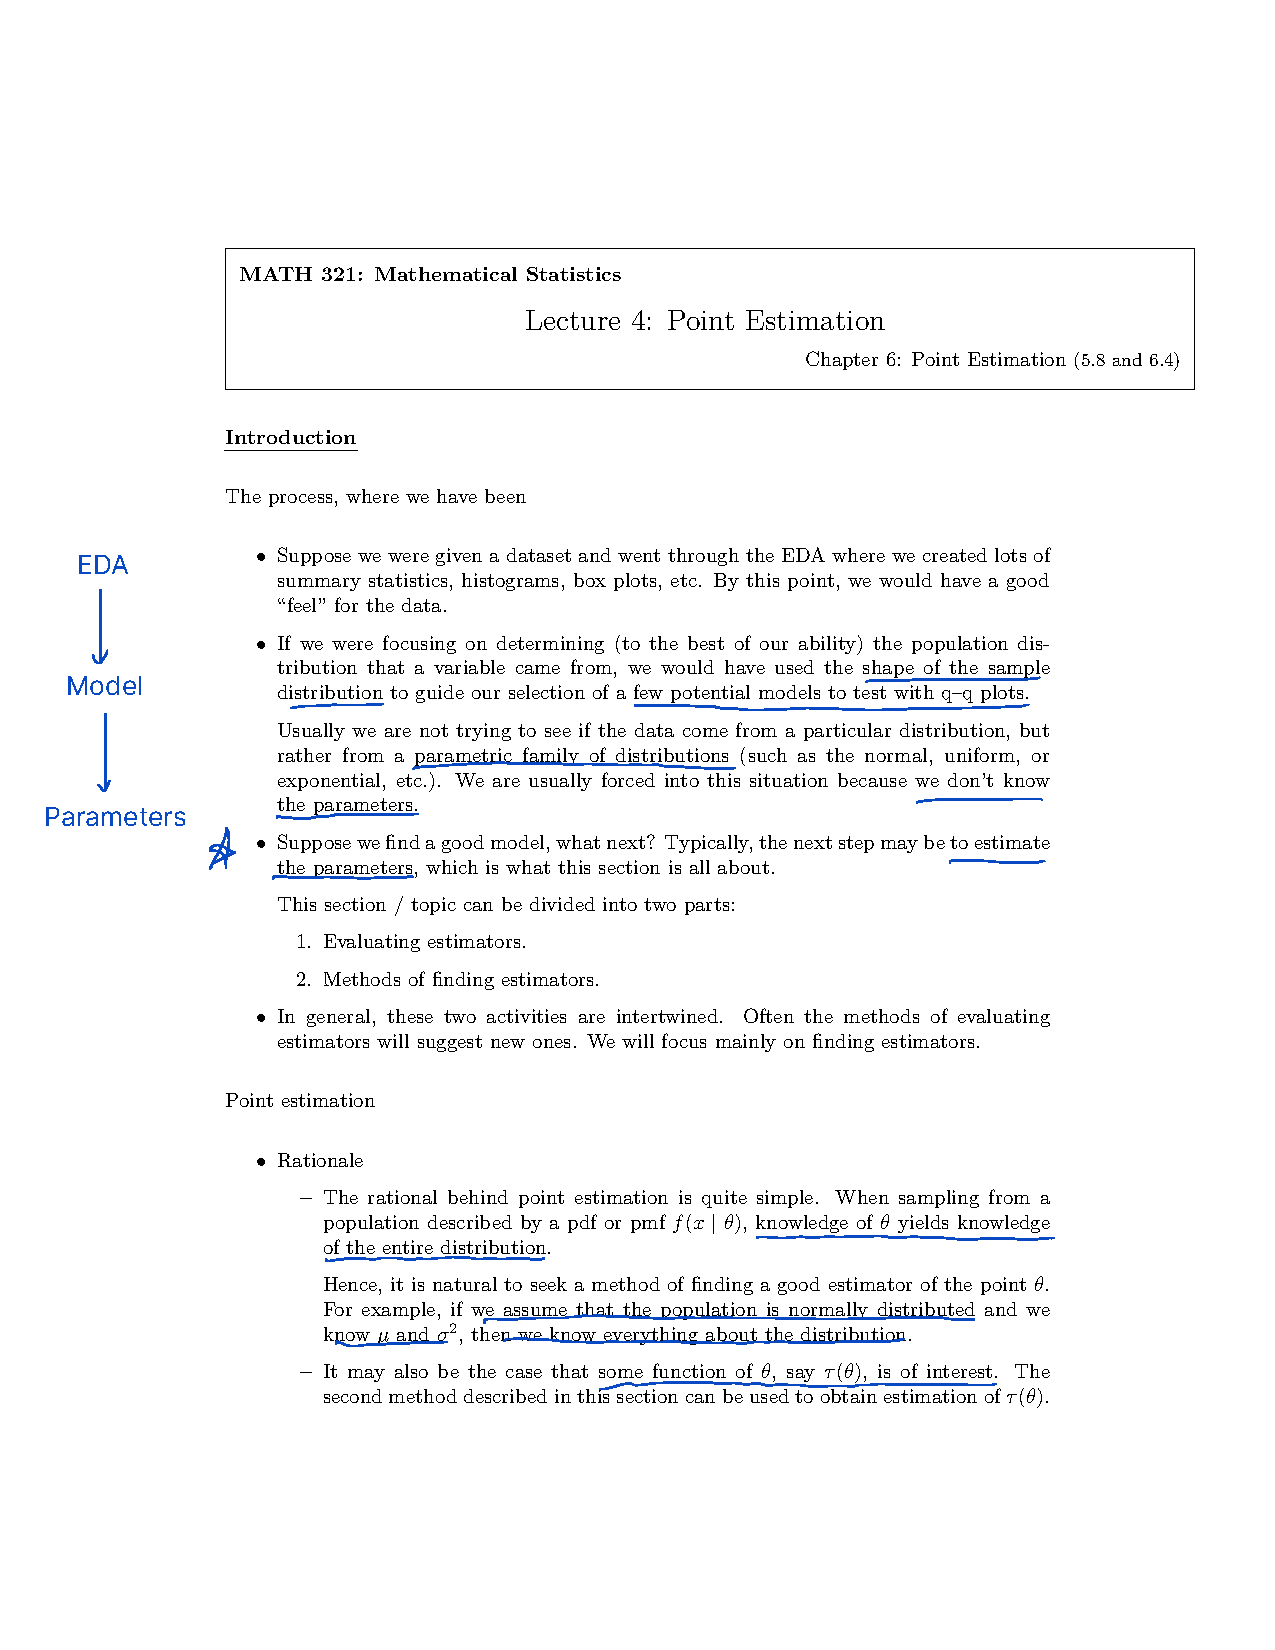
\includepdf[pages=-]{lecture-4-COMPLETED.pdf}\newpage
%%----------------------------
%
%%----------------------------
%\subsection{Lecture 5 -- XXX}
%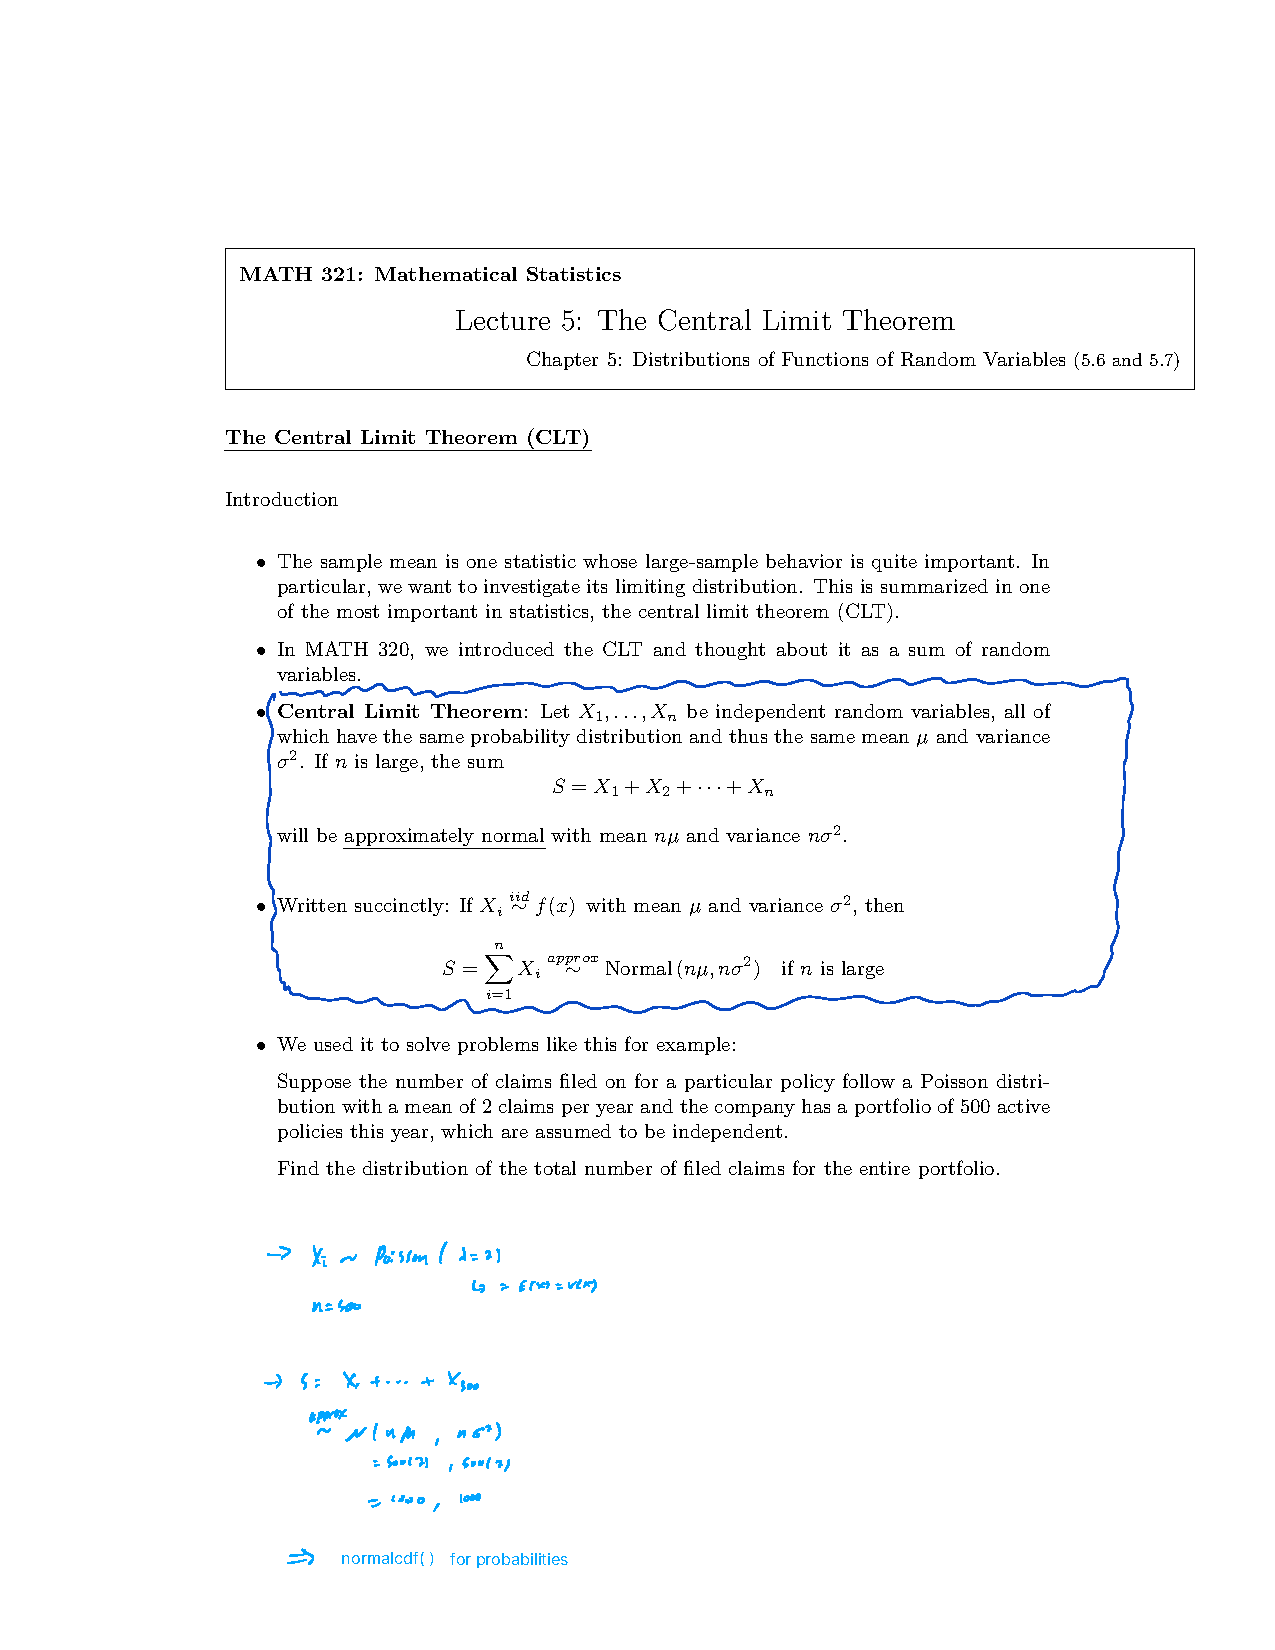
\includepdf[pages=-]{lecture-5-COMPLETED.pdf}\newpage
%%----------------------------
%
%%----------------------------
%\subsection{Lecture 6 -- XXX}
%\includepdf[pages=-]{lecture-6-COMPLETED.pdf}\newpage
%%----------------------------
%
%%-------------------------------------------------------------------------
%\section{Test 2}
%%-------------------------------------------------------------------------
%
%\secttoc
%
%%----------------------------
%\subsection{Lecture 7 -- XXX}
%\includepdf[pages=-]{lecture-7-COMPLETED.pdf}\newpage
%%----------------------------
%
%%----------------------------
%\subsection{Lecture 8 -- XXX}
%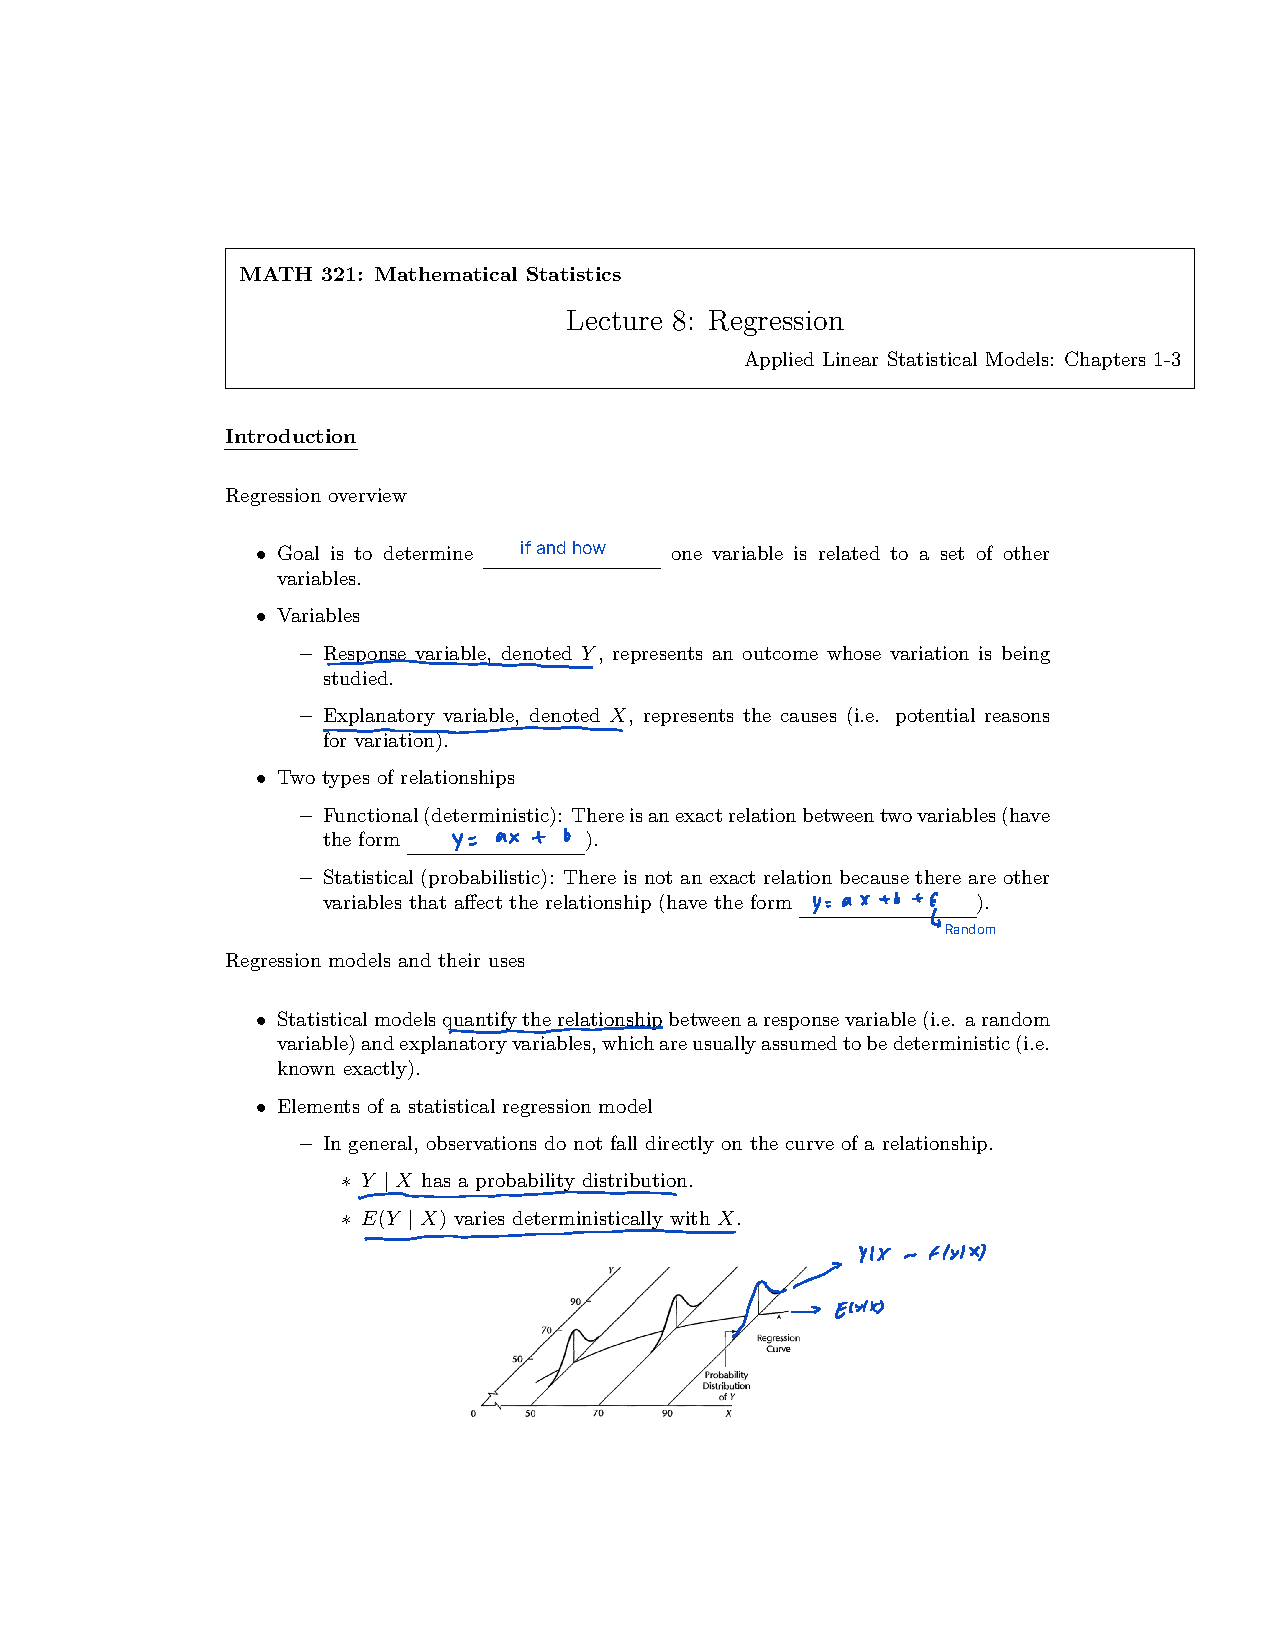
\includepdf[pages=-]{lecture-8-COMPLETED.pdf}\newpage
%%----------------------------
%
%%----------------------------
%\subsection{Lecture 9 -- XXX}
%\includepdf[pages=-]{lecture-9-COMPLETED.pdf}\newpage
%%----------------------------
%
%%-------------------------------------------------------------------------
%\section{Test 3}
%%-------------------------------------------------------------------------
%
%\secttoc
%
%%----------------------------
%\subsection{Lecture 10 -- XXX}
%\includepdf[pages=-]{lecture-10-COMPLETED.pdf}\newpage
%%----------------------------
%
%%----------------------------
%\subsection{Lecture 11 -- XXX}
%\includepdf[pages=-]{lecture-11-COMPLETED.pdf}\newpage
%%----------------------------
%
%%----------------------------
%\subsection{Lecture 12 -- XXX}
%\includepdf[pages=-]{lecture-12-COMPLETED.pdf}\newpage
%%----------------------------
%
%%-------------------------------------------------------------------------
%\section{After Test 3}
%%-------------------------------------------------------------------------
%
%\secttoc
%
%%----------------------------
%\subsection{Lecture 13 -- XXX}
%\includepdf[pages=-]{lecture-13-COMPLETED.pdf}\newpage
%%----------------------------


\end{document}